% +------------------------------------------------------------------------+
% | CGAL User Manual: 
% +------------------------------------------------------------------------+
% |
% | 10.07.2008   Peter Hachenberger
% | 
\RCSdef{\MinkowskiSum3Rev}{$Id$}
\RCSdefDate{\MinkowskiSum3Date}{$Date$}
% +------------------------------------------------------------------------+

\ccParDims

\ccUserChapter{Minkowski Sum of Polyhedra \label{chapterMinkowskiSum3}}
\ccChapterRelease{\MinkowskiSum3Rev. \ \MinkowskiSum3Date}
\ccChapterAuthor{Peter Hachenberger}

%
\begin{ccPkgDescription}{3D Convex Hulls\label{Pkg:ConvexHull3}}
\ccPkgHowToCiteCgal{cgal:hs-ch3-07}
\ccPkgSummary{This package provides functions 
for computing convex hulls in three dimensions as well as functions
for checking if sets of points are strongly convex are not. One can
compute the convex hull of a set of points in three dimensions in one
of three ways: using a static algorithm, using an incremental
construction algorithm, or using a triangulation to get a fully
dynamic computation.}

\ccPkgDependsOn{All algorithms produce as output a \ccRef[3D Polyhedron]{Pkg:Polyhedron}. 
                The dynamic algorithms depend on \ccRef[3D Triangulations]{Pkg:Triangulation3}}
\ccPkgIntroducedInCGAL{1.1}
\ccPkgLicense{\ccLicenseQPL}
\ccPkgIllustration{Convex_hull_3/bunny.png}{Convex_hull_3/bunny.png}
\end{ccPkgDescription}


% +------------------------------------------------------------------------+
\section{Introduction}

\begin{figure}[h]
  \begin{ccTexOnly}
    \begin{center}
      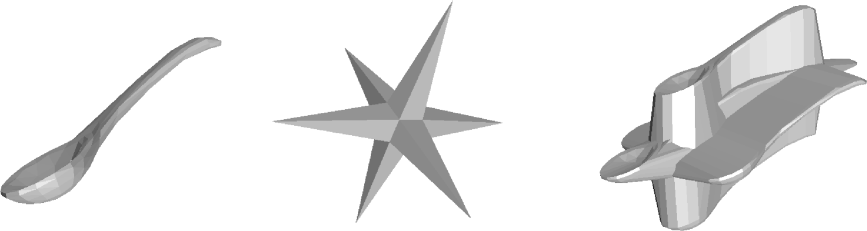
\includegraphics[width=0.8\textwidth]{Minkowski_sum_3/fig/spoon_star}
    \end{center}
  \end{ccTexOnly}
  \begin{ccHtmlOnly}
    <p><center>
    <img src="./fig/spoon_star.gif" border=0 alt="Minkowski sum example">
    </center>
  \end{ccHtmlOnly}
  \caption{The Minkowski sum of a spoon and a star.}
\end{figure}

The Minkowski sum of two point sets $P$ and $Q$ in $\mathbb{R}^d$, denoted by
$P \oplus Q$, is defined as the set $\{p+q:p \in P, q \in Q
\}$. Minkowski sums are used in a wide range of applications such as
robot motion planning and computer-aided design. This
package provides a function that computes the Minkowski sum of two Nef
polyhedra.

% +------------------------------------------------------------------------+
\section{Decomposition Method}

The decomposition method for computing the Minkowski sum of non-convex
polyhedra is based on the fact that the Minkowski sum of convex
polyhedra is rather easy to compute. The method decomposes both
polyhedra into convex pieces computes all pairwise Minkowski sums of
the convex pieces and merges the pairwise sums.

\begin{figure}
  \begin{ccTexOnly}
    \begin{center}
      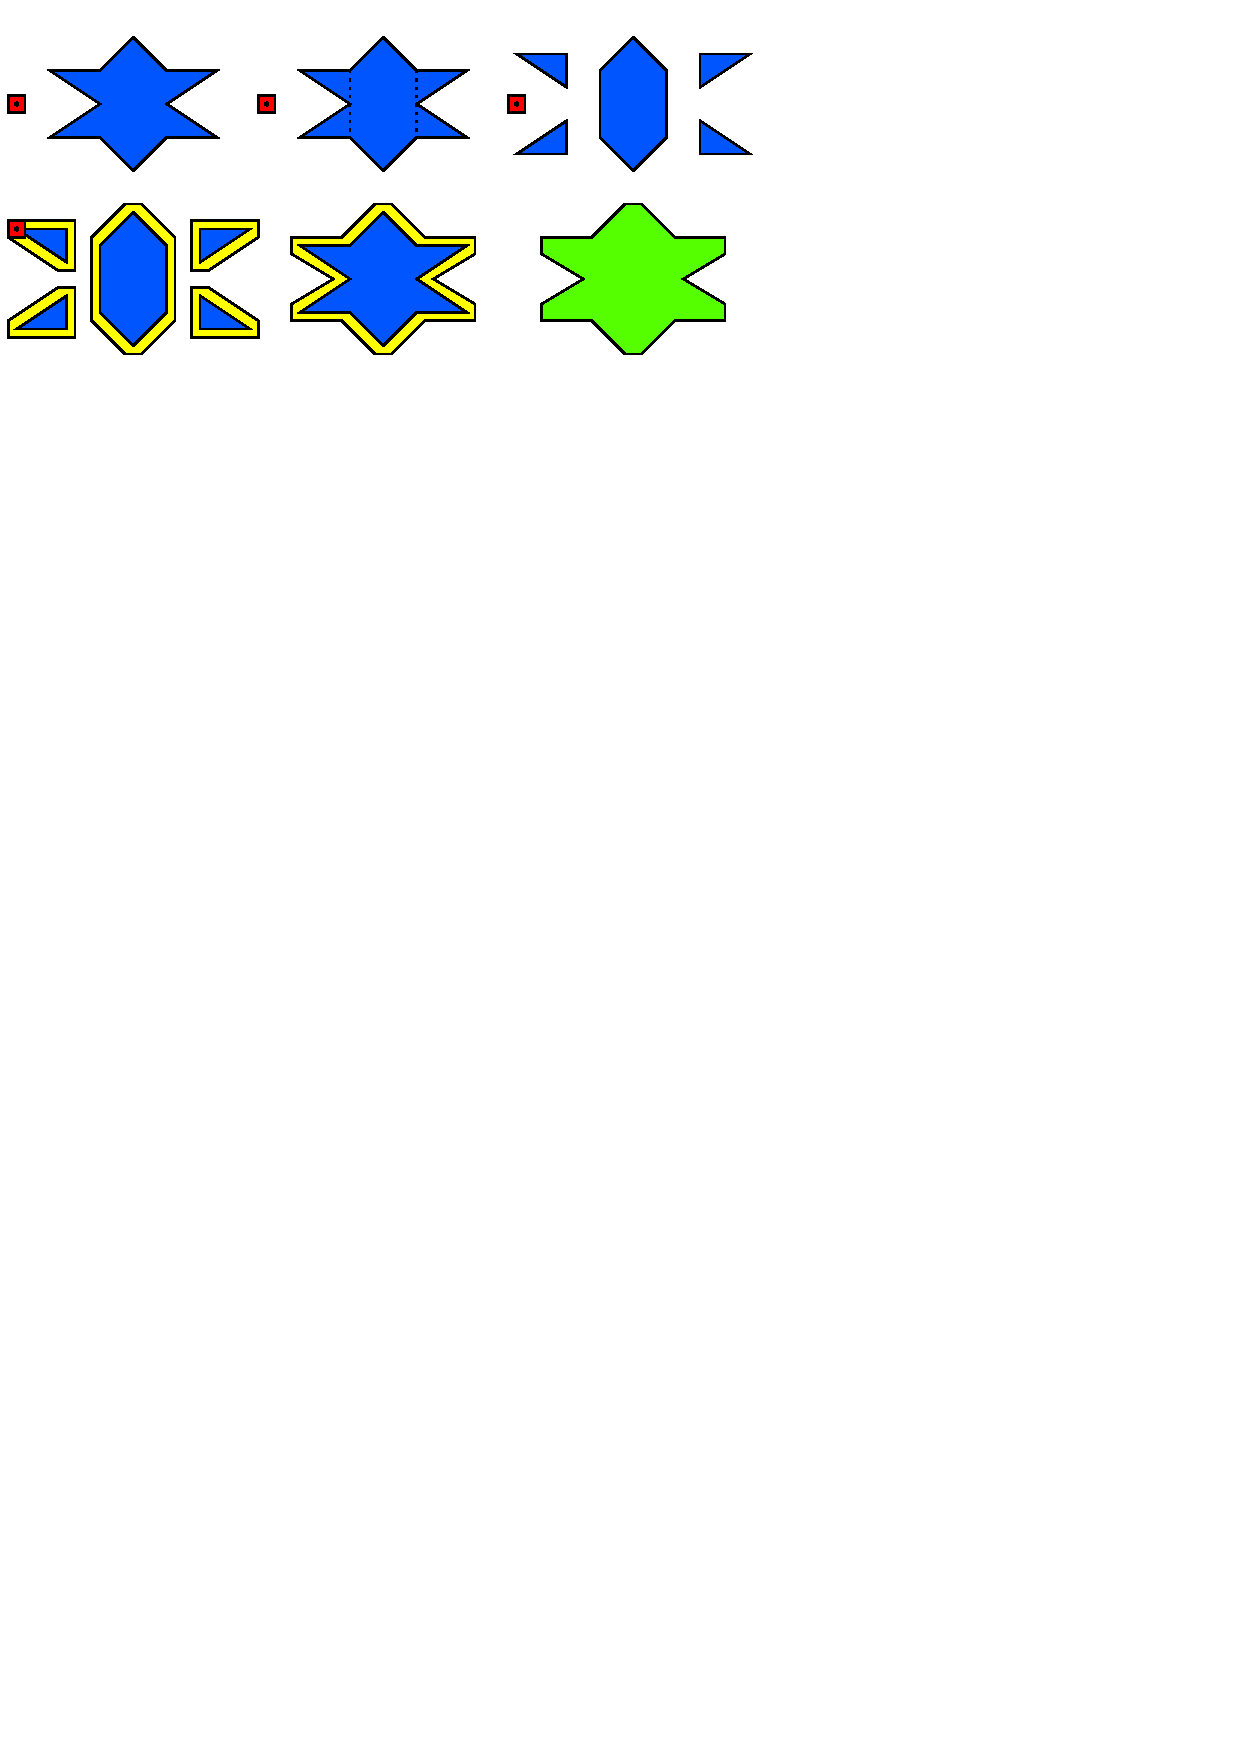
\includegraphics[width=0.8\textwidth]{Minkowski_sum_3/fig/decomposition_method}
    \end{center}
  \end{ccTexOnly}
  \begin{ccHtmlOnly}
    <p><center>
    <img src="./fig/decomposition_method.gif" border=0 alt="decomposition method">
    </center>
  \end{ccHtmlOnly}
  \caption{The decomposition method decomposes both input polyhedra
           into convex parts, computes all pairwise Minkowski sums
           of the convex parts, and merges the pairwise sums.}
\end{figure}

The Minkowski sum is an iherent complex method. Using the
decomposition method, each polyhedron might be divided into a
quadratic number of pieces, which is worst-case optimal. Then up to
$n^2m^2$ pairwise sums have to be computed and merged, where $n$ and
$m$ is the complexity of the two input polyhedra.

% +------------------------------------------------------------------------+
\section{Features and Restrictions}

This package was written to allow the computation of Minkowski sums of
full-dimensional polyhedra even in so-called tight-passage scenarios,
i.e., solve motion planing problems with passages that are exactly as
wide as the robot. In these scenarios at least one polyhedron---the
obstacles or the robot---must be modeled as an open set. This is
possible with the current implementation.

\begin{figure}
  \begin{ccTexOnly}
    \begin{center}
      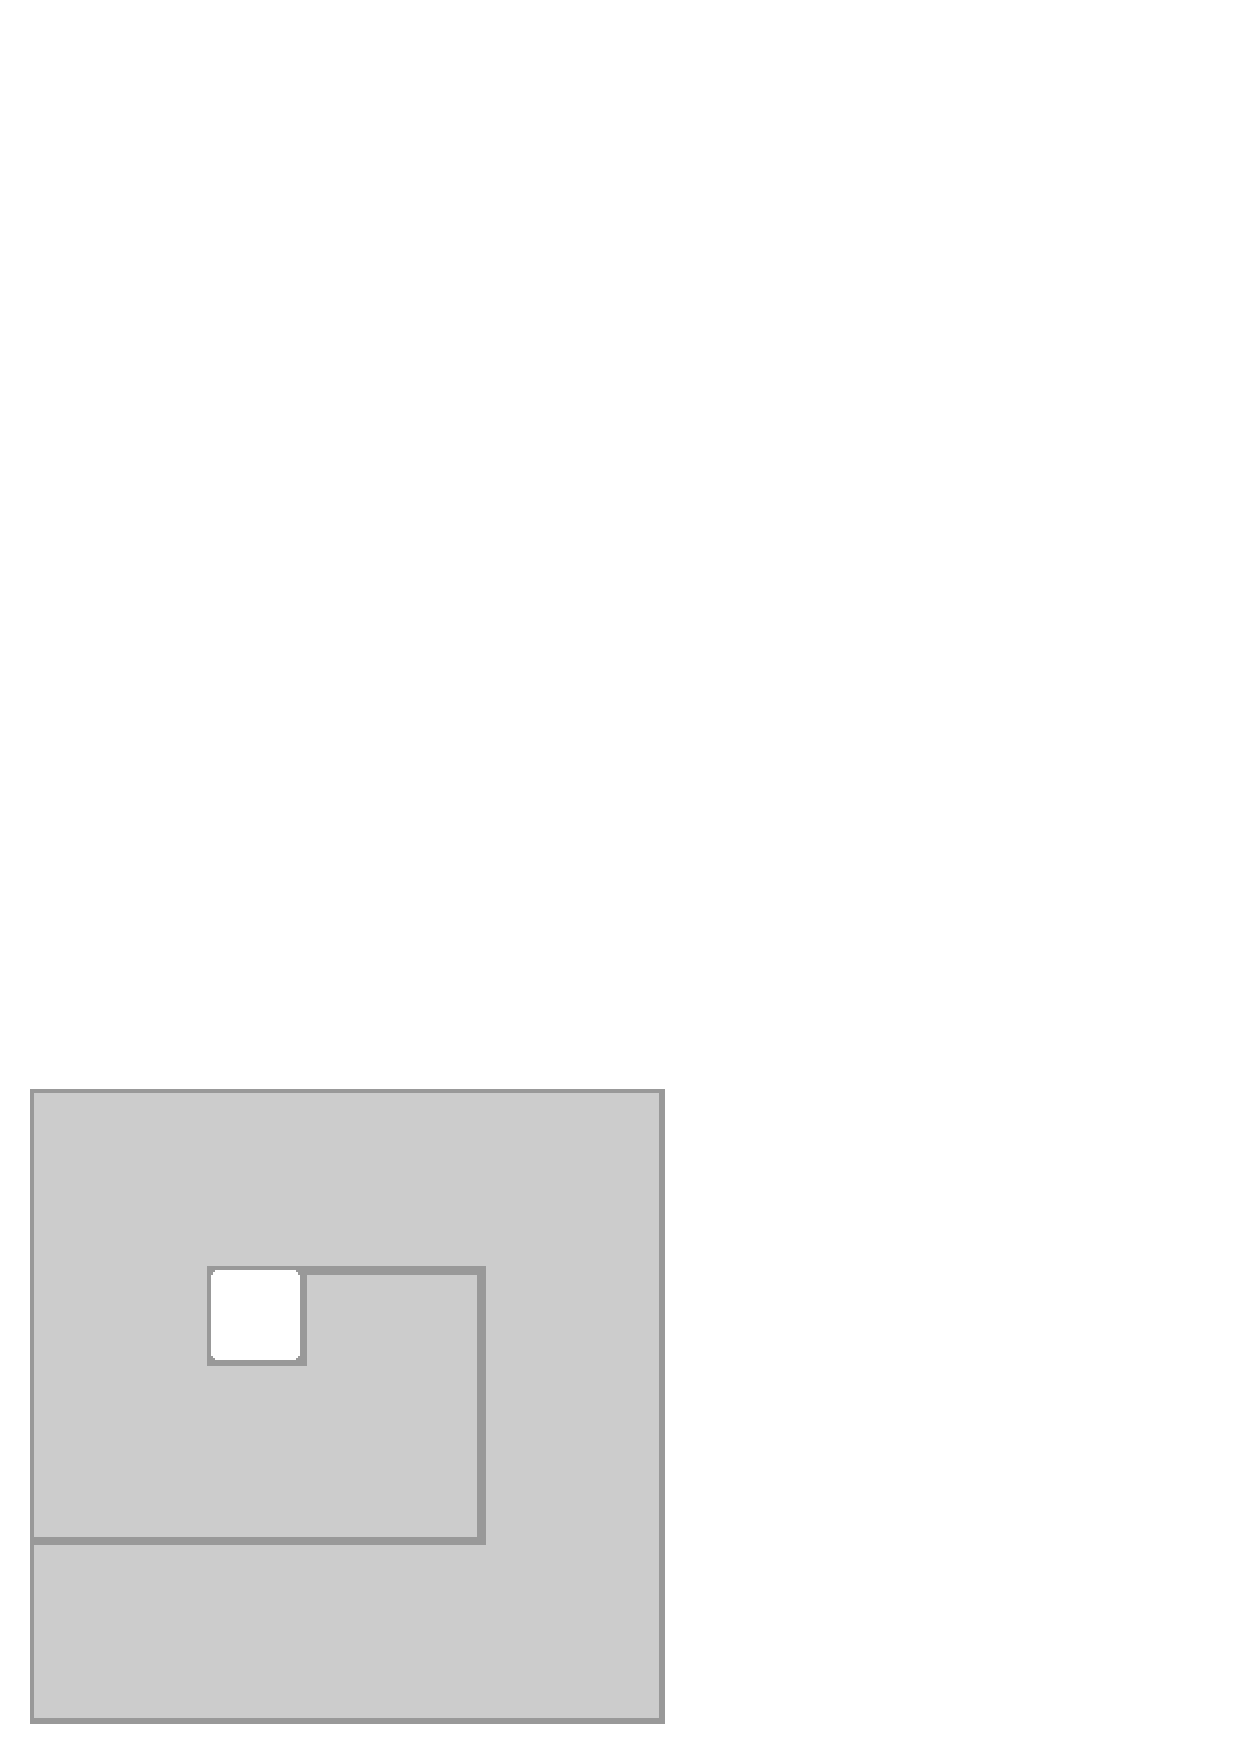
\includegraphics[width=0.5\textwidth]{Minkowski_sum_3/fig/tight_passage}
    \end{center}
  \end{ccTexOnly}
  \begin{ccHtmlOnly}
    <p><center>
    <img src="./fig/tigh_passage.gif" border=0 alt="tight passage">
    </center>
  \end{ccHtmlOnly}
  \caption{The Minkowski sum of a maze and a cube that exactly fits through
	   the corridor of the maze. Modeling the cube as an open set, the
	   Minkowski sum includes facets that represent the remaining path
           for the cubical robot.}
\end{figure}

We strife for extending the package to work for arbitrary
polyhedra. Yet we added several features, but are not complete. At
the moment we allow an input polyhedron to consist of:
\begin{enumerate}
\item singular vertices
\item singular edges
\item singular convex facets without holes
\item surface with convex facets that have no holes.
\item open or closed solids
\end{enumerate}

Taking a different viewpoint, the implementation is restricted as
follows:
\begin{enumerate}
\item The input polyhedra must be finite point sets.
\item Every convex Minkowski sum must be full-dimensional, i.e., one 
of the two input polyhedra must not include lower-dimensional
featueres. Note that lower-dimensional holes are still possible.
\item All sets of coplanar facets that form a side of a full-dimensional
featuer, must have the same selection mark.
\item All facets of lower-dimensional features need to be convex and 
must not have holes.
\end{enumerate}

% +------------------------------------------------------------------------+
\section{Usage}

The following example code illustrates the usage of the function
\ccc{minkowski_sum_3}. Note that the two input polyhedra will be
destroyed by the function. So, if they are further on needed, they
need to be copied, first. The copying is not done by the function
itself to keep the memory usage as small as possible.

\ccIncludeExampleCode{Minkowski_sum_3/cube_offset.cpp}

% +------------------------------------------------------------------------+
\section{Glide}

\begin{figure}
  \begin{ccTexOnly}
    \begin{center}
      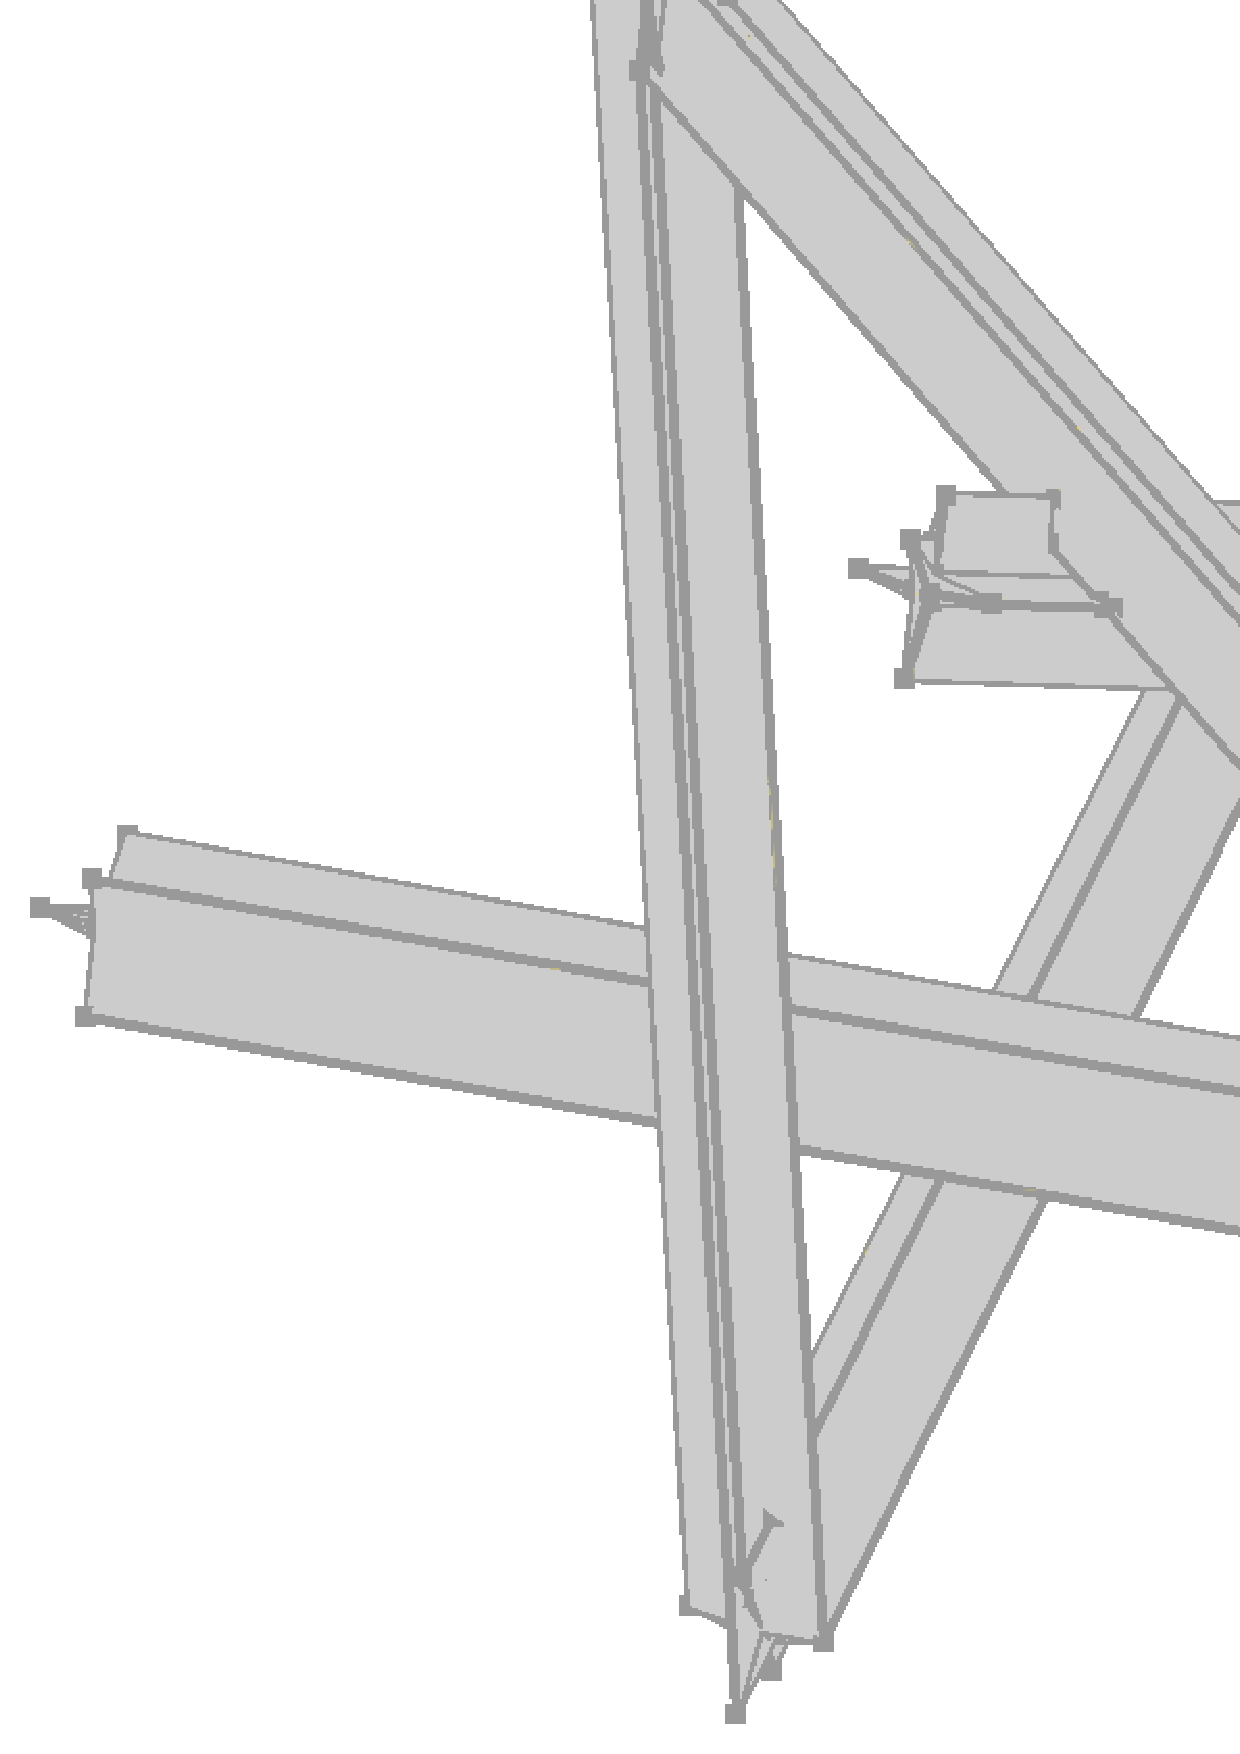
\includegraphics[width=0.5\textwidth]{Minkowski_sum_3/fig/glide}
    \end{center}
  \end{ccTexOnly}
  \begin{ccHtmlOnly}
    <p><center>
    <img src="./fig/glide.gif" border=0 alt="glide operation">
    </center>
  \end{ccHtmlOnly}
  \caption{The region swept by a star that moves along a polygonal path.}
\end{figure}

With the function \ccc{minkowski_sum_3} it is also possible to realize
other interesting geometric operations like glide operation, which
computes the point set swept by polyhedron that moves along a
polygonal path. The following example shows how to construct a
polygonal path and then compute the glide operation by calling the
function \ccc{minkowski_sum_3}.

\ccIncludeExampleCode{Minkowski_sum_3/glide.cpp}
